\documentclass[compress,aspectratio=169]{beamer}

\usetheme{Singapore}

\beamertemplatenavigationsymbolsempty
\setbeamertemplate{bibliography item}[text]

%http://tex.stackexchange.com/a/50003/9115
\makeatletter
\setbeamertemplate{footline}
{
  \leavevmode%
  \hbox{%
  \begin{beamercolorbox}[wd=.25\paperwidth,ht=2.25ex,dp=2ex,left]{author in head/foot}%
    \usebeamerfont{author in
head/foot}%
  \hspace*{2ex}%
  \insertshortauthor%\hspace{1em}\beamer@ifempty{\insertshortinstitute}{}{(\insertshortinstitute)}
  \end{beamercolorbox}%
  \begin{beamercolorbox}[wd=.5\paperwidth,ht=2.25ex,dp=2ex,center]{title in head/foot}%
    \usebeamerfont{title in head/foot}\insertshorttitle
  \end{beamercolorbox}%
  \begin{beamercolorbox}[wd=.25\paperwidth,right]{date in head/foot}%
    \usebeamerfont{date in head/foot}\insertshortdate{}%\hspace*{2em}
    %\insertframenumber{} / \inserttotalframenumber%
    \hspace*{2ex} 
  \end{beamercolorbox}}%
  \vskip0pt%
}
\makeatother

%http://tex.stackexchange.com/a/66626/9115
\usepackage{etoolbox}
\makeatletter
\patchcmd{\slideentry}{\ifnum#2>0}{\ifnum2>0}{}{\@error{unable to patch}}% replace the subsection number test with a test that always returns true
%http://tex.stackexchange.com/a/132312/9115
% use frame numbers instead of subsection slide numbers so that frames broken over slides get separate circles
\patchcmd{\slideentry}{\c@subsectionslide}{\c@framenumber}{}{\@error{unable to patch}}
\patchcmd{\beamer@writeslidentry}{\c@subsectionslide}{\c@framenumber}{}{\@error{unable to patch}}
\makeatother

%http://tex.stackexchange.com/a/45038/9115
\makeatletter
\let\beamer@writeslidentry@miniframeson=\beamer@writeslidentry
\def\beamer@writeslidentry@miniframesoff{%
  \expandafter\beamer@ifempty\expandafter{\beamer@framestartpage}{}% does not happen normally
  {%else
    % removed \addtocontents commands
    \clearpage\beamer@notesactions%
  }
}
\newcommand*{\miniframeson}{\let\beamer@writeslidentry=\beamer@writeslidentry@miniframeson}
\newcommand*{\miniframesoff}{\let\beamer@writeslidentry=\beamer@writeslidentry@miniframesoff}
\makeatother

\usepackage{helvet}
\renewcommand\mathfamilydefault{cmr} % ss for sans serif

\usepackage{hyperref}
\usepackage{graphicx}
\usepackage{tikz}
\usetikzlibrary{chains, trees}

\usepackage[british]{babel}
\usepackage[utf8]{inputenc}

\usepackage{tgpagella}
\usepackage[defaultmono]{droidmono}
\usepackage[T1]{fontenc}

\usepackage{amsmath, calc, seqsplit}

\usepackage{fancyvrb}
\RecustomVerbatimEnvironment{Verbatim}{Verbatim}{fontsize=\small,tabsize=4,numbers=left}

\title[Public Key Cryptography \& Public Key Infrastructure]{Public Key Cryptography \& Public Key Infrastructure\\\large and How They Apply to Code Signing \& Provisioning Profiles}
\subtitle{\#{}puggerslecture}
\author{Nicholas Helke}
\institute{Kaldor Ltd}
\subject{Brown Bag}

\begin{document}

{
\setbeamertemplate{headline}{\pgfuseshading{beamer@headfade}}
{
\setbeamertemplate{footline}{}
\frame{\titlepage}
}
\frame{\frametitle{Summary}\tableofcontents}
}

\section{Introduction}

\begin{frame}[fragile]{Alice and Bob}
\begin{center}
\begin{tikzpicture}[
    start chain=going right,
    diagram item/.style={
        on chain,
        join
    },
    scale=0.8, every node/.style={transform shape}
]

\node [
    diagram item,
    label=below:Alice
] {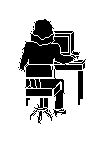
\includegraphics[scale=1.33]{macwoman}};

\node [
    diagram item,
    label=center:Internet
] {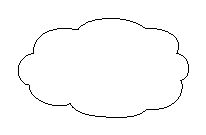
\includegraphics{cloud}};

\node [
	start branch=2 going below,
    diagram item,
    label=below:NSA
] {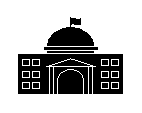
\includegraphics{governmentbuilding}};

\node [
    diagram item,
    label=below:Bob
] {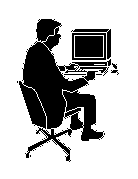
\includegraphics{pcman}};

\end{tikzpicture}
\end{center}
\end{frame}

\begin{frame}{Caesar Cipher}
Caesar cipher is an extremely basic symmetric-key algorithm. Here is an example with a shift of $k=-1\equiv 25\mod 26$ :
\begin{equation*}
\begin{matrix}
\cdots & \texttt{Z} & \texttt{A} & \texttt{B} & \texttt{C} & \cdots & \texttt{I} & \cdots & \texttt{M} & \cdots\\
& \downarrow & \downarrow & \downarrow & \downarrow && \downarrow && \downarrow\\
\cdots & \texttt{Y} & \texttt{Z} & \texttt{A} & \texttt{B} & \cdots & \texttt{H} & \cdots & \texttt{L} & \cdots
\end{matrix}
\end{equation*}
With the above shift, {\tt IBM} becomes {\tt HAL}.
\end{frame}

\begin{frame}{Asymmetric-Key Cryptography}
A simple real-world analogy for asymmetric-key algorithms:
\begin{enumerate}
\item Bob gives Alice an open padlock $K$ for which only he has the key $k$
\item Alice puts her message in a secure case and locks it with Bob's padlock $K$
\item Alice sends it to Bob, safe in the knowledge that the NSA cannot open it
\item Bob receives the secure case and opens it using his key $k$
\end{enumerate}
\end{frame}

\begin{frame}{Man-in-the-middle Attack}
\begin{enumerate}
\item Bob gives Alice an open padlock $K$ for which only he has the key $k$
\item\label{mitm:enum:intercept} The NSA intercepts $K$ and replaces it with $K_{\mathrm{NSA}}$
\item Alice puts her message in a secure case and locks it with what she believes to be Bob's padlock $K_{\mathrm{NSA}}$
\item Alice sends it to Bob, thinking that the NSA cannot open it
\item The NSA intercepts Alice's message to Bob, decrypt it with their private key $k_{\mathrm{NSA}}$, reencrypt it using Bob's public key $K$ (obtained in step~\ref{mitm:enum:intercept}), and pass it on to Bob.
\item Bob receives the secure case and opens it using his key $k$, thinking that the message safely made it to him without interception
\end{enumerate}
\end{frame}

\section{Public Key Cryptography}

\begin{frame}{Modular Arithmetic}
$\mathbb{Z}_5$ for example:
\begin{align}
0 \equiv 0\cdot 5 + 0 &\equiv 0 \mod 5\\
1 \equiv 0\cdot 5 + 1 &\equiv 1 \mod 5\\
2 \equiv 0\cdot 5 + 2 &\equiv 2 \mod 5\\
3 \equiv 0\cdot 5 + 3 &\equiv 3 \mod 5\\
4 \equiv 0\cdot 5 + 4 &\equiv 4 \mod 5\\
5 \equiv 1\cdot 5 + 0 &\equiv 0 \mod 5\\
6 \equiv 1\cdot 5 + 1 &\equiv 1 \mod 5\\
                      &\mathrel{\makebox[\widthof{$\equiv$}]{\vdots}} \nonumber
\end{align}
\end{frame}

\begin{frame}[allowframebreaks]{RSA}
The fundamental building block of RSA is Euler's theorem which asserts
\begin{equation}
a^{\phi(n)} \equiv a^0\equiv 1 \mod n\label{eq:rsa:euler}
\end{equation}
if $a$ and $n$ are coprime.

\framebreak

RSA works by selecting a private key $k$ and a public key $K$ such that:
\begin{equation}
kK = \phi(n)+1
\end{equation}
If we combine this with Euler's theorem (\ref{eq:rsa:euler}) we get
\begin{equation}
a^{k^K} \equiv a^{\phi(n)+1} \equiv a^1\equiv a \mod n
\end{equation}
where $a$ is the message to be ecrypted.

\framebreak

The first step to creating an RSA key-pair is to select $n$ and determine $\phi(n)$. Given a random $n$ it is generally not feasable to compute $\phi(n)$. (It has exponential time-complexity in the general case.) Using the following two properties of Euler's totient function we can choose a number $n$ such that we can determine $\phi(n)$ cheaply:
\begin{eqnarray}
\phi(p) = p-1&\text{if $p$ is prime}\\
\phi(pq) = \phi(p)\phi(q)
\end{eqnarray}

\framebreak

So we select two primes $p=3$ and $q=11$:
\begin{eqnarray}
n = pq = 3\cdot 11 = 33\\
\phi(n) = \phi(pq) = \phi(p)\phi(q) = (3-1)(11-1) = 20
\end{eqnarray}

If we don't reveal $p$ or $q$ and only ever reveal $n$ there is no cheap way of computing $\phi(n)$.

\framebreak

Using the extended Euclidian algorithm we find $k = 7$ and $K = 3$ such that:
\begin{equation}
kK = 7\cdot 3 = 21 = \phi(n)+1
\end{equation}

We now announce to the world that our public key is $K=3$ and that we use $n=33$.

We keep all other variables secret as the security of RSA depends on it.

\framebreak

Alice now wishes to send $a=8$ to Bob so she computes:
\begin{equation}
a^K \equiv 8^3 \equiv 512\equiv 17 \mod 33
\end{equation}
Bob receives $a^K\equiv 17\mod 33$ from Alice and decrypts it with his private key:
\begin{equation}
\left(a^K\right)^k \equiv 17^7 \equiv 410338673\equiv 8\equiv a\mod 33
\end{equation}
\end{frame}

\begin{frame}[fragile]{My Public Key}
\begin{align}
n &= %
\underbrace{
\begin{minipage}[c]{10.4cm}
\tiny
\seqsplit{$
828484404626825435850982412881346202026638776262892403825867990564122606233869541456427400040356459584784876478571524492957655454238457362846848372246491989535738064449977403469034474411699429506841276149808122552703578859761389174527261579508183802748075016150521395764037500914794509803888427198038918600957075727493264532128266473910551413761885221004807103101749977314574494422723486652601271467774311061491811403616670936412665673151452302498097993063060422431707195593373773451887312192560879559791329409614807199327873012851675770767548405866504899854851827538713303332170620823613684520310223902610300040481931949787894719828479157450284805904668252698132775099910146925799864632235729603269993532248964170422601955162005999651902031036716683343463460481703726185841471828674133406219214645274205713682283154195878034052755688351825096734480536517175547430087895762716432821069119669862028044475907671264374904845097058824148177266270236181914413713966305678323728520607887982635316931062520198674553833473602176829413330899196249287297173459636159937649329776460467745718571460268748506125058155268938280998162530008610876181485767006215740541230175504165461890260836895055444578268695465887479939935286939848175459030773987
$}
\end{minipage}
}_{\text{1233 digits or 4096 bits}}\\
K &= 65537
\end{align}

\end{frame}

\section{Public Key Infrastructure}

{
\frame{\centering\Large\structure{How do I share my public key with you\\ without the NSA intercepting it and replacing it?}}
}

\begin{frame}[allowframebreaks]{Digital Signature}
Exponentiation is commutative:
\begin{equation}
\left(a^k\right)^K\Leftrightarrow \left(a^K\right)^k
\end{equation}
This means that RSA can just as easily be used to digitally sign content.

\framebreak

Bob wishes to send Alice an application. Alice is prepared to trust the code Bob wrote, but wants to be sure when she receives the application that it hasn't been tampered with enroute by the NSA. 

Bob encrypts his app $a=8$ with his private key and posts it on a webpage.
\begin{equation}
a^k \equiv 8^7 \equiv 2097152\equiv 2 \mod 33
\end{equation}
Alice or anyone for that matter can see $a^k\equiv 2\mod 33$ on Bob's webpage and decrypt it with his public key:
\begin{equation}
\left(a^k\right)^K \equiv 2^3 \equiv 8\equiv a\mod 33
\end{equation}
\end{frame}

\begin{frame}{Certificate}
\centering\Large A certificate is a public key signed by a trusted private key.
\end{frame}

\begin{frame}[fragile]{Trust chain}
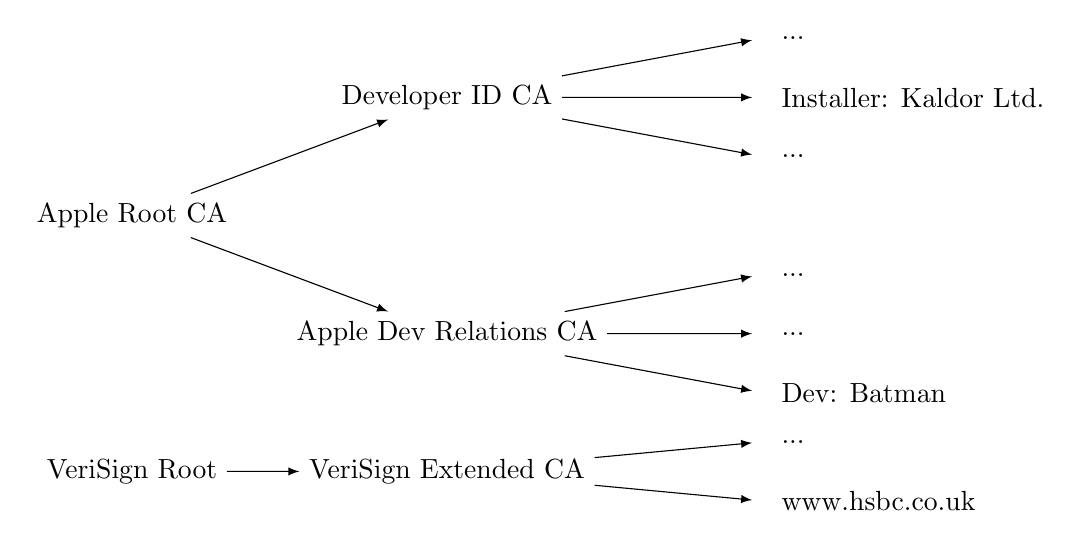
\begin{tikzpicture}[grow=right, sloped,
level 1/.style={level distance=4cm, sibling distance=3cm},
level 2/.style={level distance=4cm, sibling distance=0.75cm},
edge from parent/.style={black,->,>=latex,draw}
]
\node (apple) {Apple Root CA}
    child {
      node {Apple Dev Relations CA}        
          child {
            node [label=right:{Dev: Batman}] {}
            edge from parent
          }
          child {
            node [label=right:{...}] {}
            edge from parent
          }
          child {
            node [label=right:{...}] {}
            edge from parent
          }
          edge from parent 
    }
    child {
      node {Developer ID CA}
          child {
              node [label=right:{...}] {}
            edge from parent
          }
          child {
            node [label=right:{Installer: Kaldor Ltd.}] {}
            edge from parent
          }
          child {
              node [label=right:{...}] {}
              edge from parent
          }
          edge from parent
    };
\node[below of=apple, node distance=3.25cm]{VeriSign Root}
    child {
      node {VeriSign Extended CA}        
          child {
            node [label=right:{www.hsbc.co.uk}] {}
            edge from parent
          }
          child {
            node [label=right:{...}] {}
            edge from parent
          }
          edge from parent 
    };
\end{tikzpicture}
\end{frame}

\section{Entr'acte}

\begin{frame}{In Summary}
\begin{enumerate}
\item Symetric-Key Cryptography
\item Public-Key Cryptography
\item Digital Signing
\item Certificates
\item Trust Chain
\end{enumerate}
\end{frame}

{
\frame{\centering\Huge\structure{Entr'acte}}
}

\section{Code Signing and Provisioning Profiles}

\begin{frame}{Code signing}
\begin{enumerate}
\item All modern platforms use code signing to guard against malicious code and code modification.
\item Even desktops are starting to embrace this with UEFI secure boot, for instance.
\item iOS devices only run code that has been signed by Apple (or someone Apple has said they trust by signing their key)
\end{enumerate}
\end{frame}

\begin{frame}{Provisioning Profiles}
\begin{enumerate}
\item A provisioning profile associates a bundle ID with authorised certificates, entitlements and devices.
\item Apple signs the provisioning profile.
\item Only code signed by Apple or code with a valid provisioning profile will run on an iOS device.
\end{enumerate}
\end{frame}

\begin{frame}{Xcode Weirdness}
Ever wonder why Xcode asks you for provisioning profile twice?
\begin{enumerate}
\item Builds {\tt .app}, embeds profile into binary and copies profile to {\tt .app/embedded.mobileprovision}
\item Copies {\tt .app} into {\tt Payload} folder, replaces {\tt Payload/*.app/embedded.mobileprovision} with the user selected profile and ZIPs the result up to form an IPA
\end{enumerate}
If the two profiles do not match, Testflight calls this ``mismatched keychain-access-groups''.
\end{frame}

\begin{frame}{Conclusion}
\begin{enumerate}
\item Symetric-Key Cryptography
\item Public-Key Cryptography
\item Digital Signing
\item Certificates
\item Trust Chain
\item Code Signing
\item Provisioning Profiles
\end{enumerate}
\end{frame}

\miniframesoff
{
\setbeamertemplate{headline}{\pgfuseshading{beamer@headfade}}
\frame{\centering\Huge\structure{Thank you}}
}

\end{document}
